\section{Sensitivity of the Rust Model}
\thispagestyle{plain} % surpress header on first page

As described in section \ref{generalMPEC}, the economic literature exploring the benefits of MPEC and NFXP for structural estimation is limited to studies by \cite{Su.Judd.2012}, \cite{Dube.Fox.Su.2012}, \cite{Jorgensen.2013}, \cite{Iskhakov.2016} and \cite{Dong.Hsieh.Zhang.2017}. While in these papers different economic models are considered, the set up chosen is quite clean, being mainly free of any model misspecification and allowing mostly for stable, small numerical errors in the calibration procedure. From a practical perspective and in a research setting where economic models and calibration procedures become more complex, a comparison of MPEC and NFXP is inherently limited to a world in which the modeling and calibration procedure is performed with a minimal error. In a more realistic set up that practioners commonly face where their mathematical model might be more or less off from reality and the computational model has to work with many approximations, there might actually be a larger difference between the two approaches. Those studies comparing the two approaches unanimously find that the qualitative results, i.e. the parameter estimates are the same for both which is why they focus on the implementation side covering the speed and rate of convergence. The idea of my following simulation study is to break with the clean comparison of MPEC and NFXP by deliberately introducing some numerical error and model misspecification to test how the two approaches react to it. In this comparison I focus on qualitative aspects investigating how well the two approaches calibrate the model. For this a first aspect of the UQ framework comes into play. As I will also change the level of model misspecification in the Rust model a naive comparison of how the structural parameters of the underlying data generating process are recovered, as done by \cite{Su.Judd.2012}, is flawed. For this reason I rely on the previously used QoI of the counterfactual demand level at replacement cost of 11,000 Dollars. This quantity can be calculated and compared no matter the degree of model misspecification and it is an indicator on how well certain parameters in combination with some model and numerical specifications actually uncovers the predictions of the true underlying model and data generating process. A second aspect from uncertainty quantification that enters my following simulation study is the general framework of \cite{Oberkampf.2010}. They devise an approach for scientific computing in which they account for model and numerical error as well as parameter uncertainty and propagate them in various combinations through a model resulting in many different distributions of a QoI that in the end is visualized such that it is informative about the uncertainty in the QoI for those that intend to actually use the model outcome. In my simulation study I pick up key ideas of this framework and consequently investigate how changes in model specification and numerical implementation in the calibration procedure translate into the distribution of a QoI and hence its uncertainty. I do so by performing a large scale Monte Carlo simulation for the Rust model which is well explored and therefore can be seen as the perfect benchmark for such a study whose results might probably be taken as a lower bound for the effects in modern and much more complex structural models.

\subsection{The Simulation Setup}


\begin{figure}[H]
	\caption{Distribution of the QoI}
	\vspace*{-4mm}
	\centering
	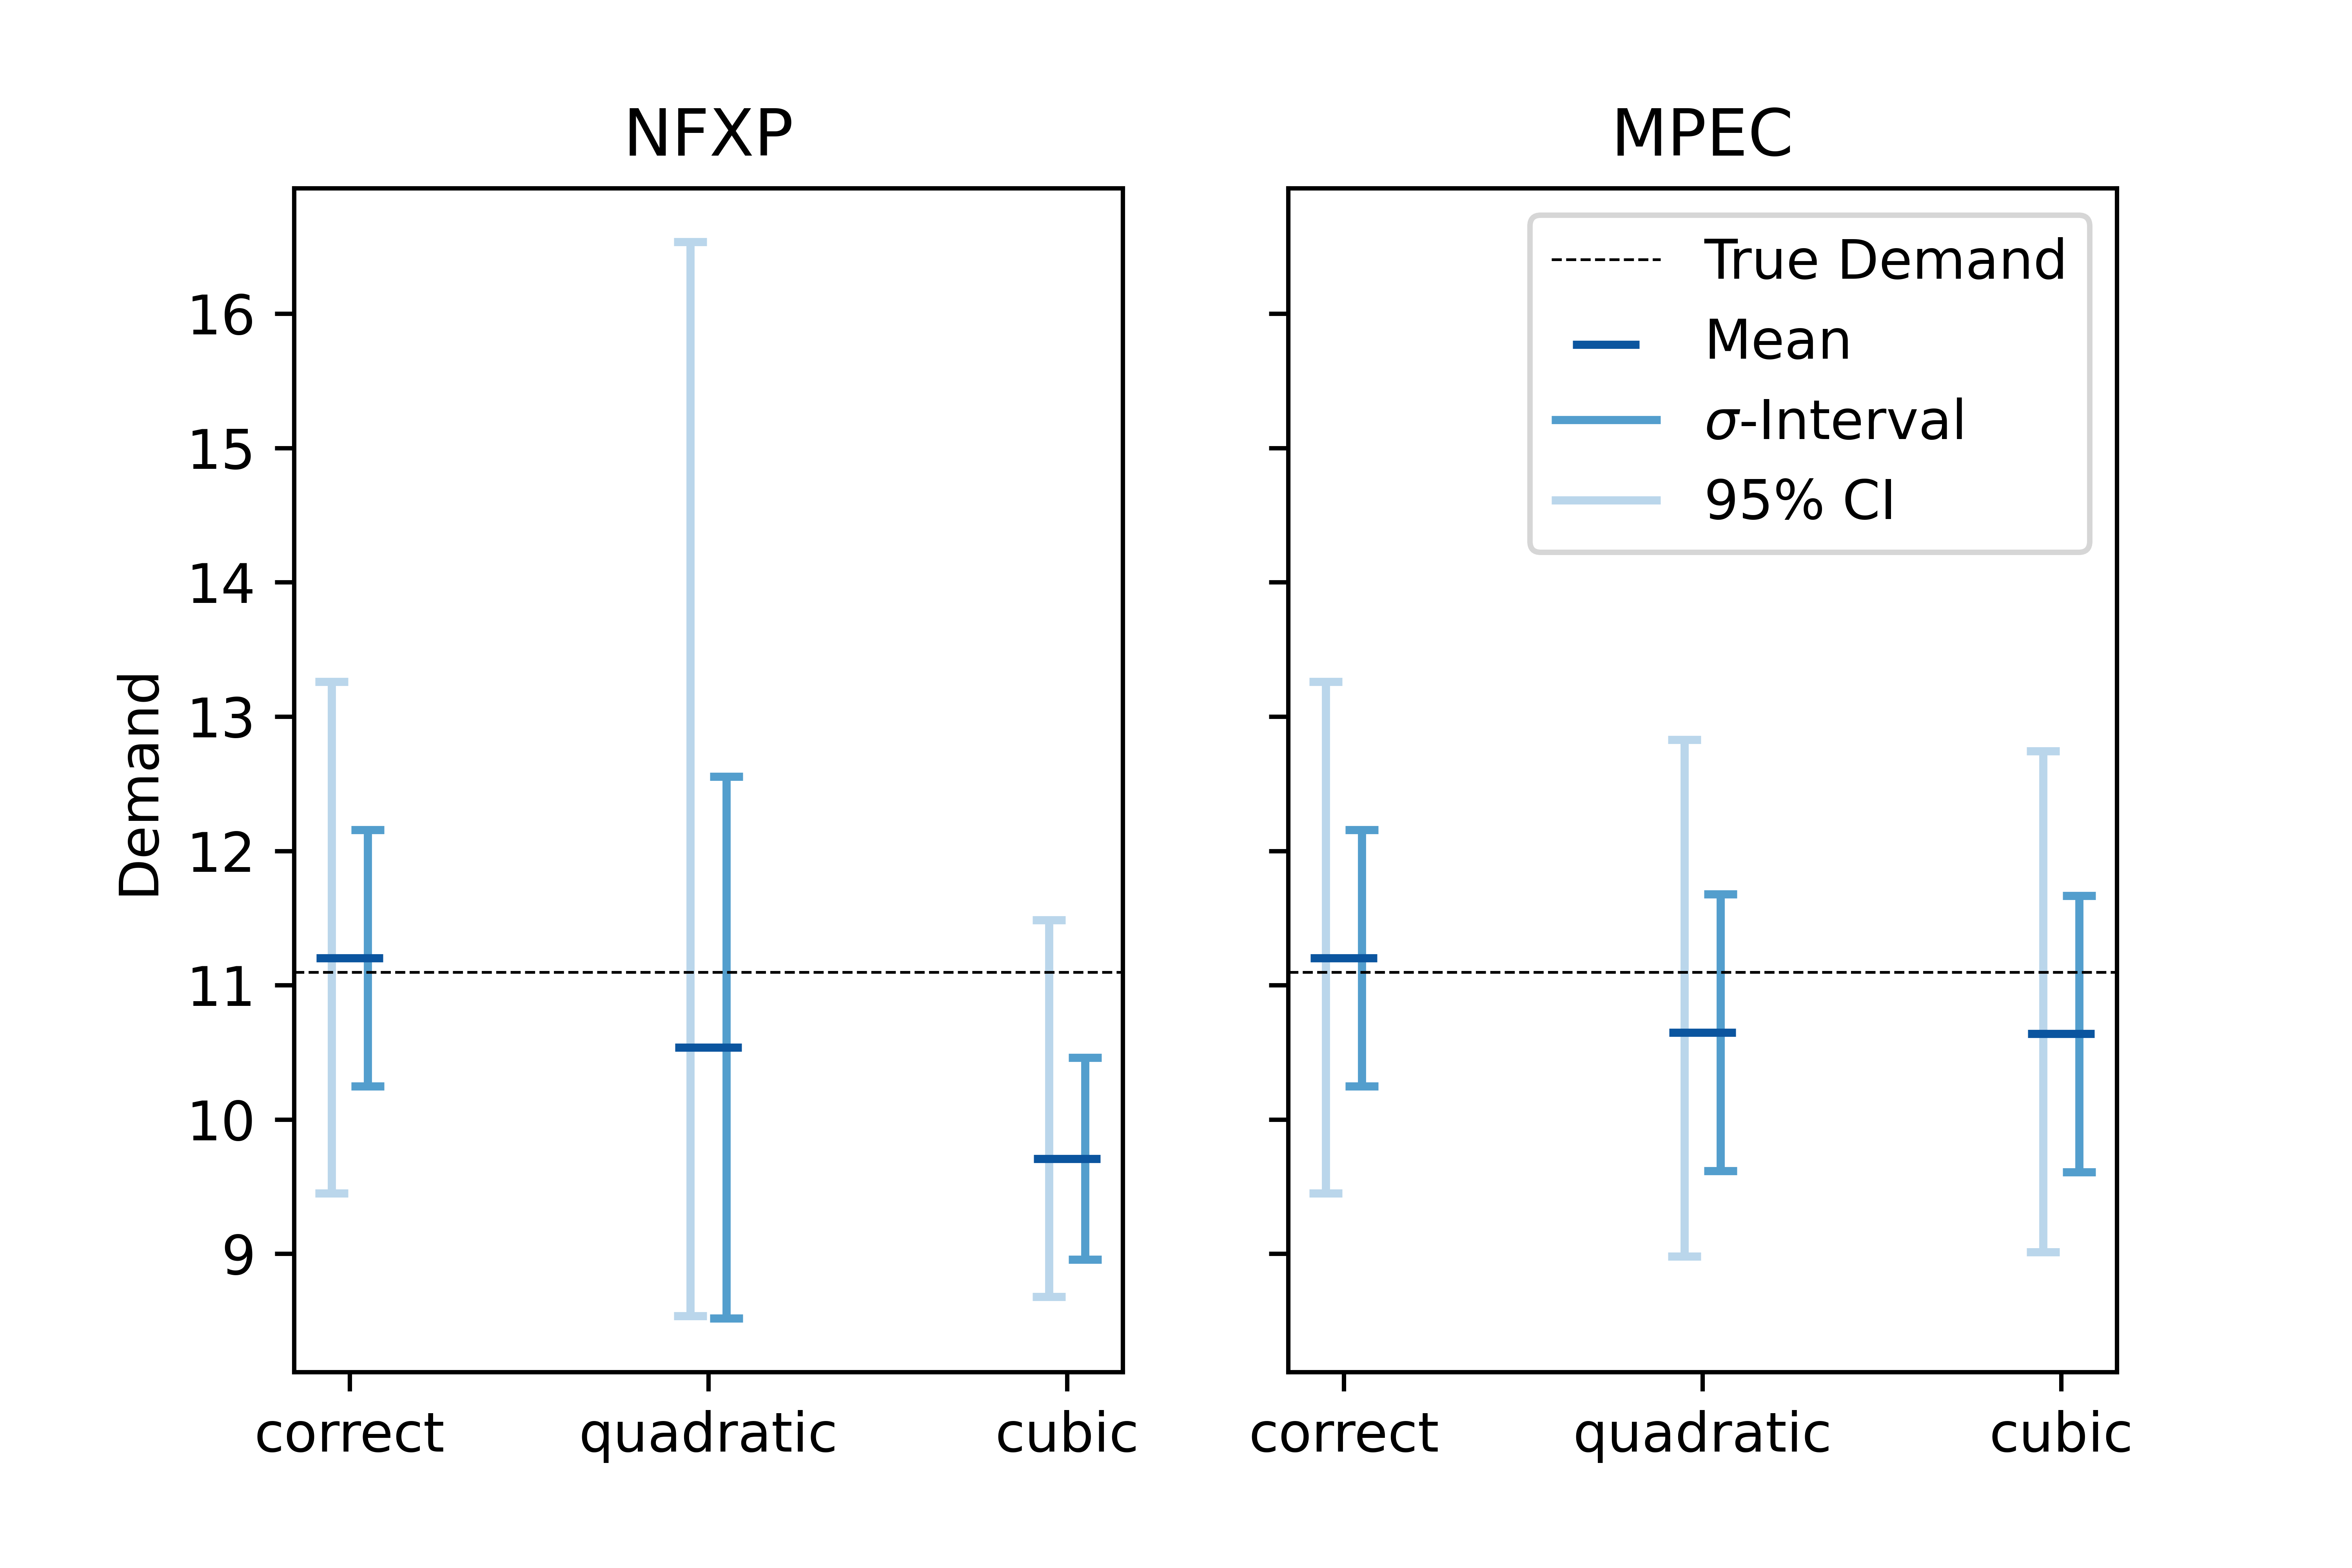
\includegraphics[scale=0.9]{../figures/figure_5.png}
	\label{figure5}
\end{figure}


\begin{figure}[H]
	\caption{Distribution of the QoI}
	\vspace*{-4mm}
	\centering
	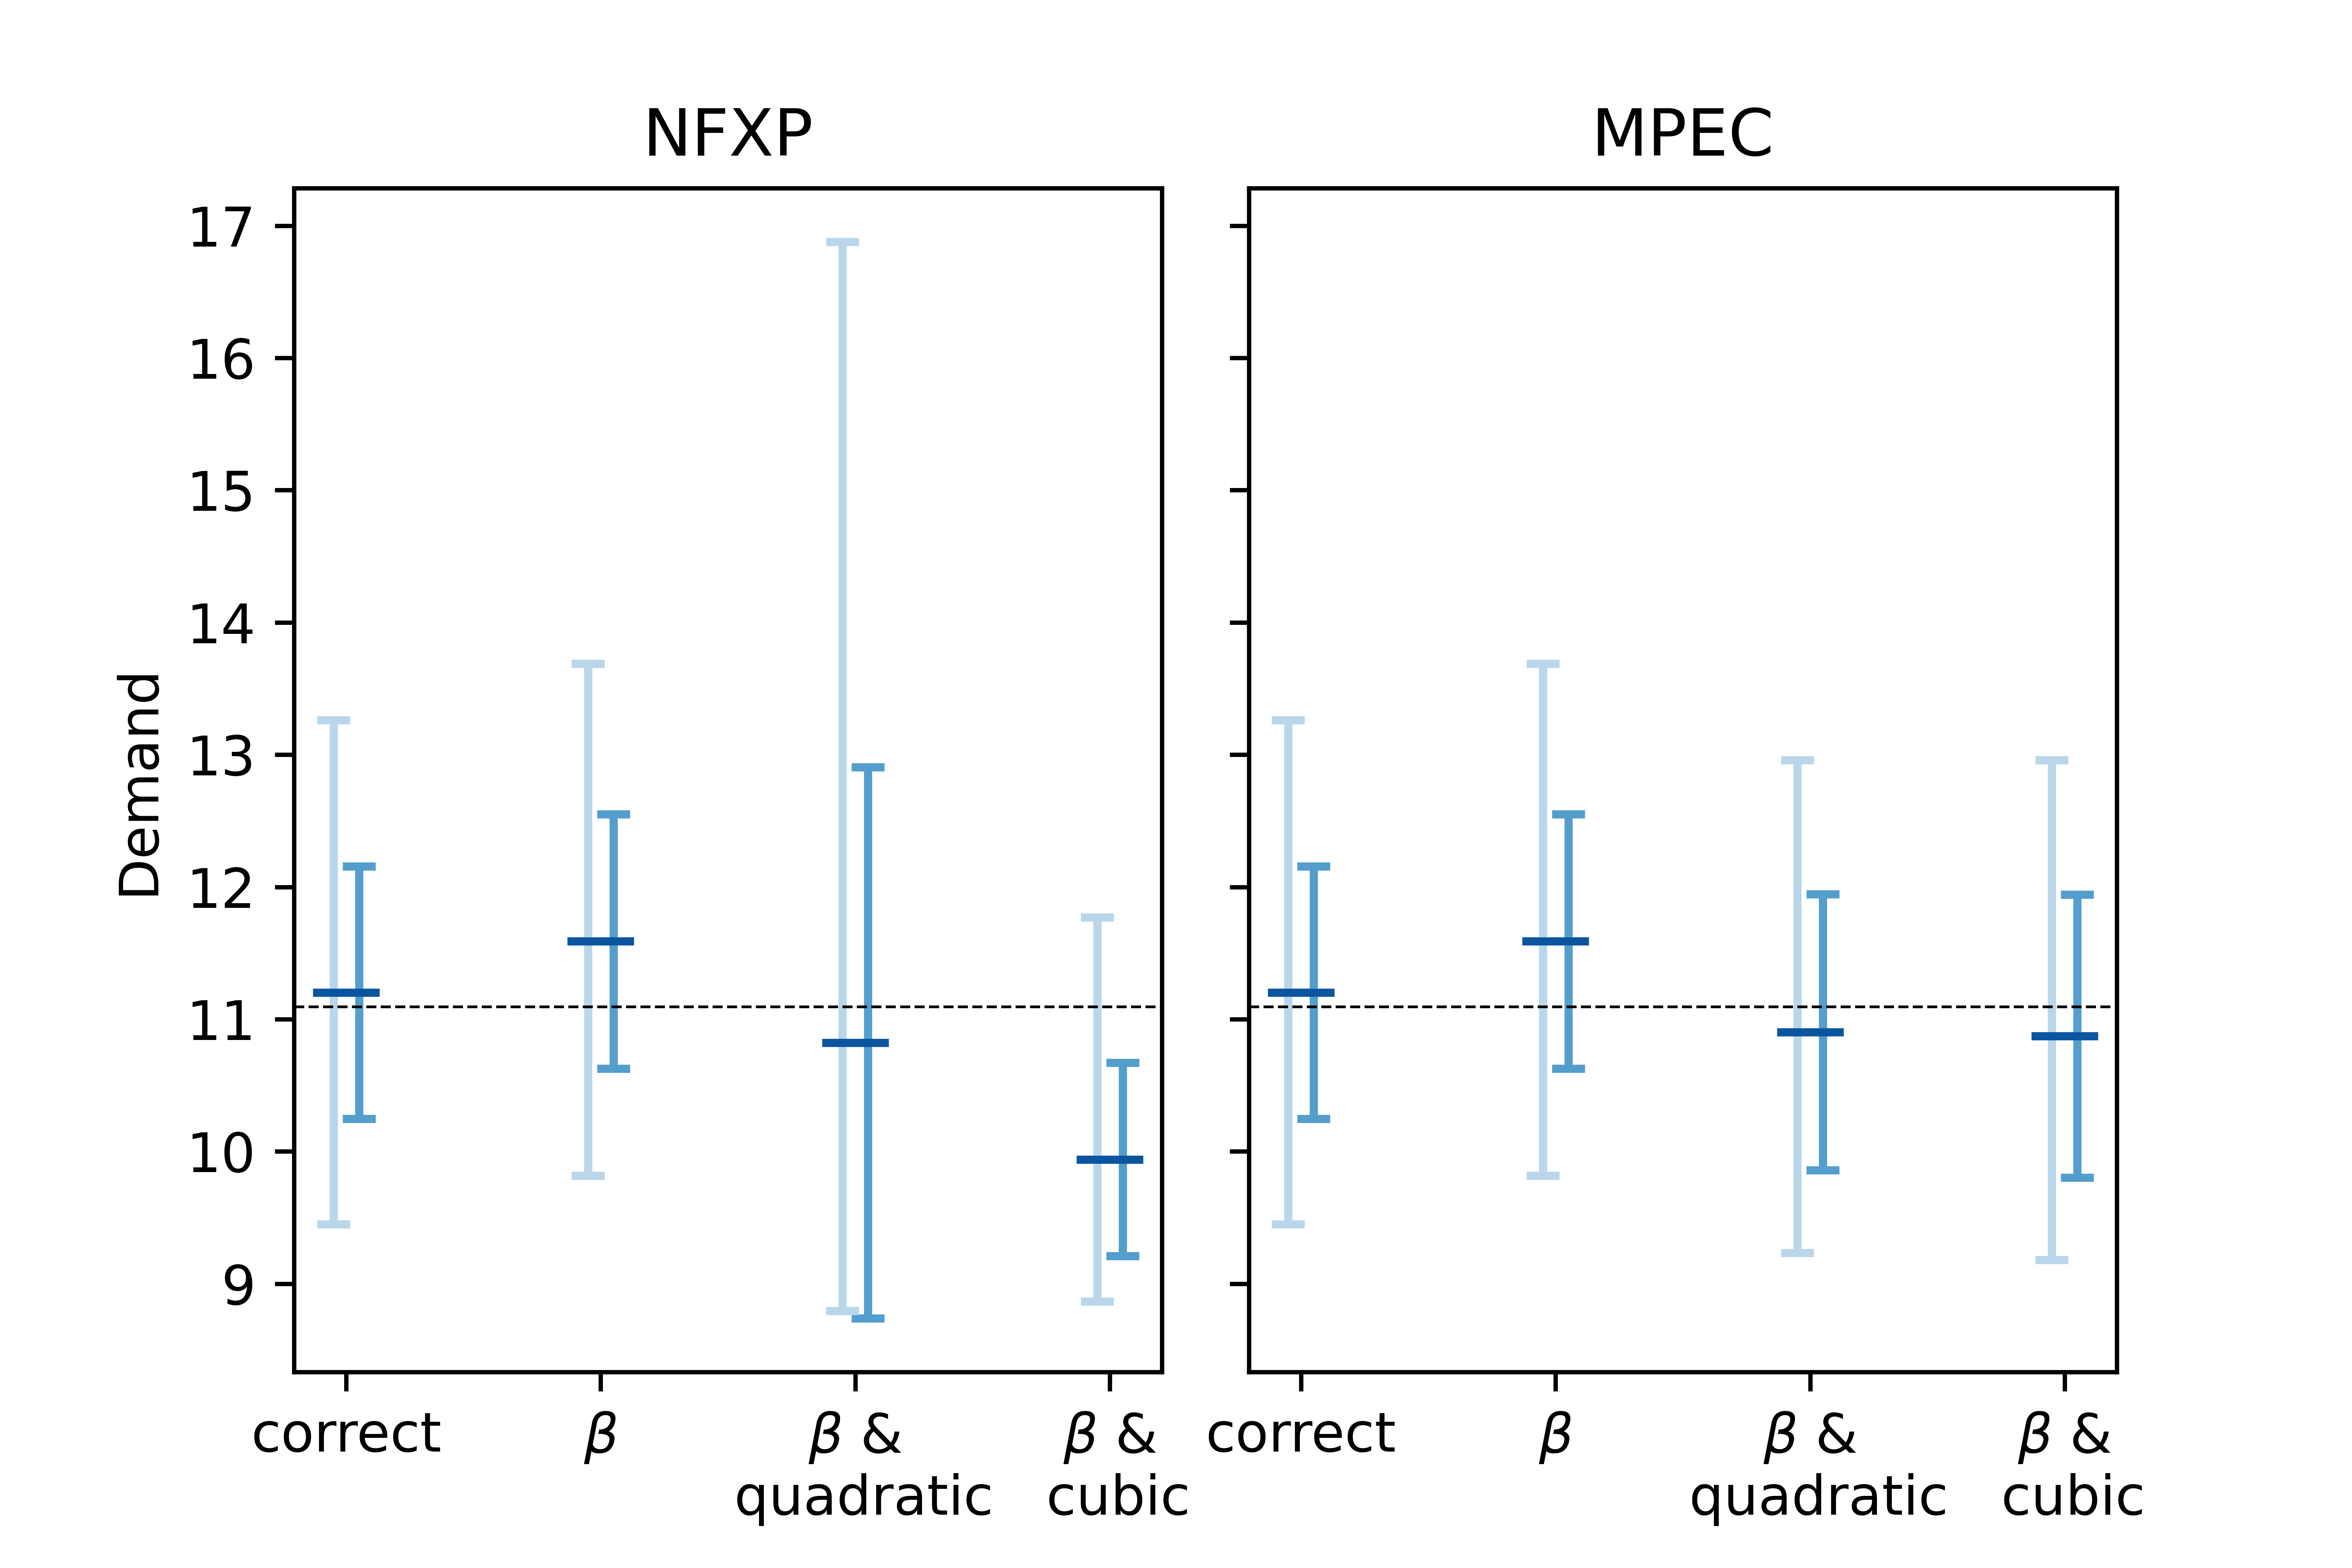
\includegraphics[scale=0.9]{../figures/figure_6.png}
	\label{figure6}
\end{figure}

\begin{figure}[H]
	\caption{Distribution of the QoI}
	\vspace*{-4mm}
	\centering
	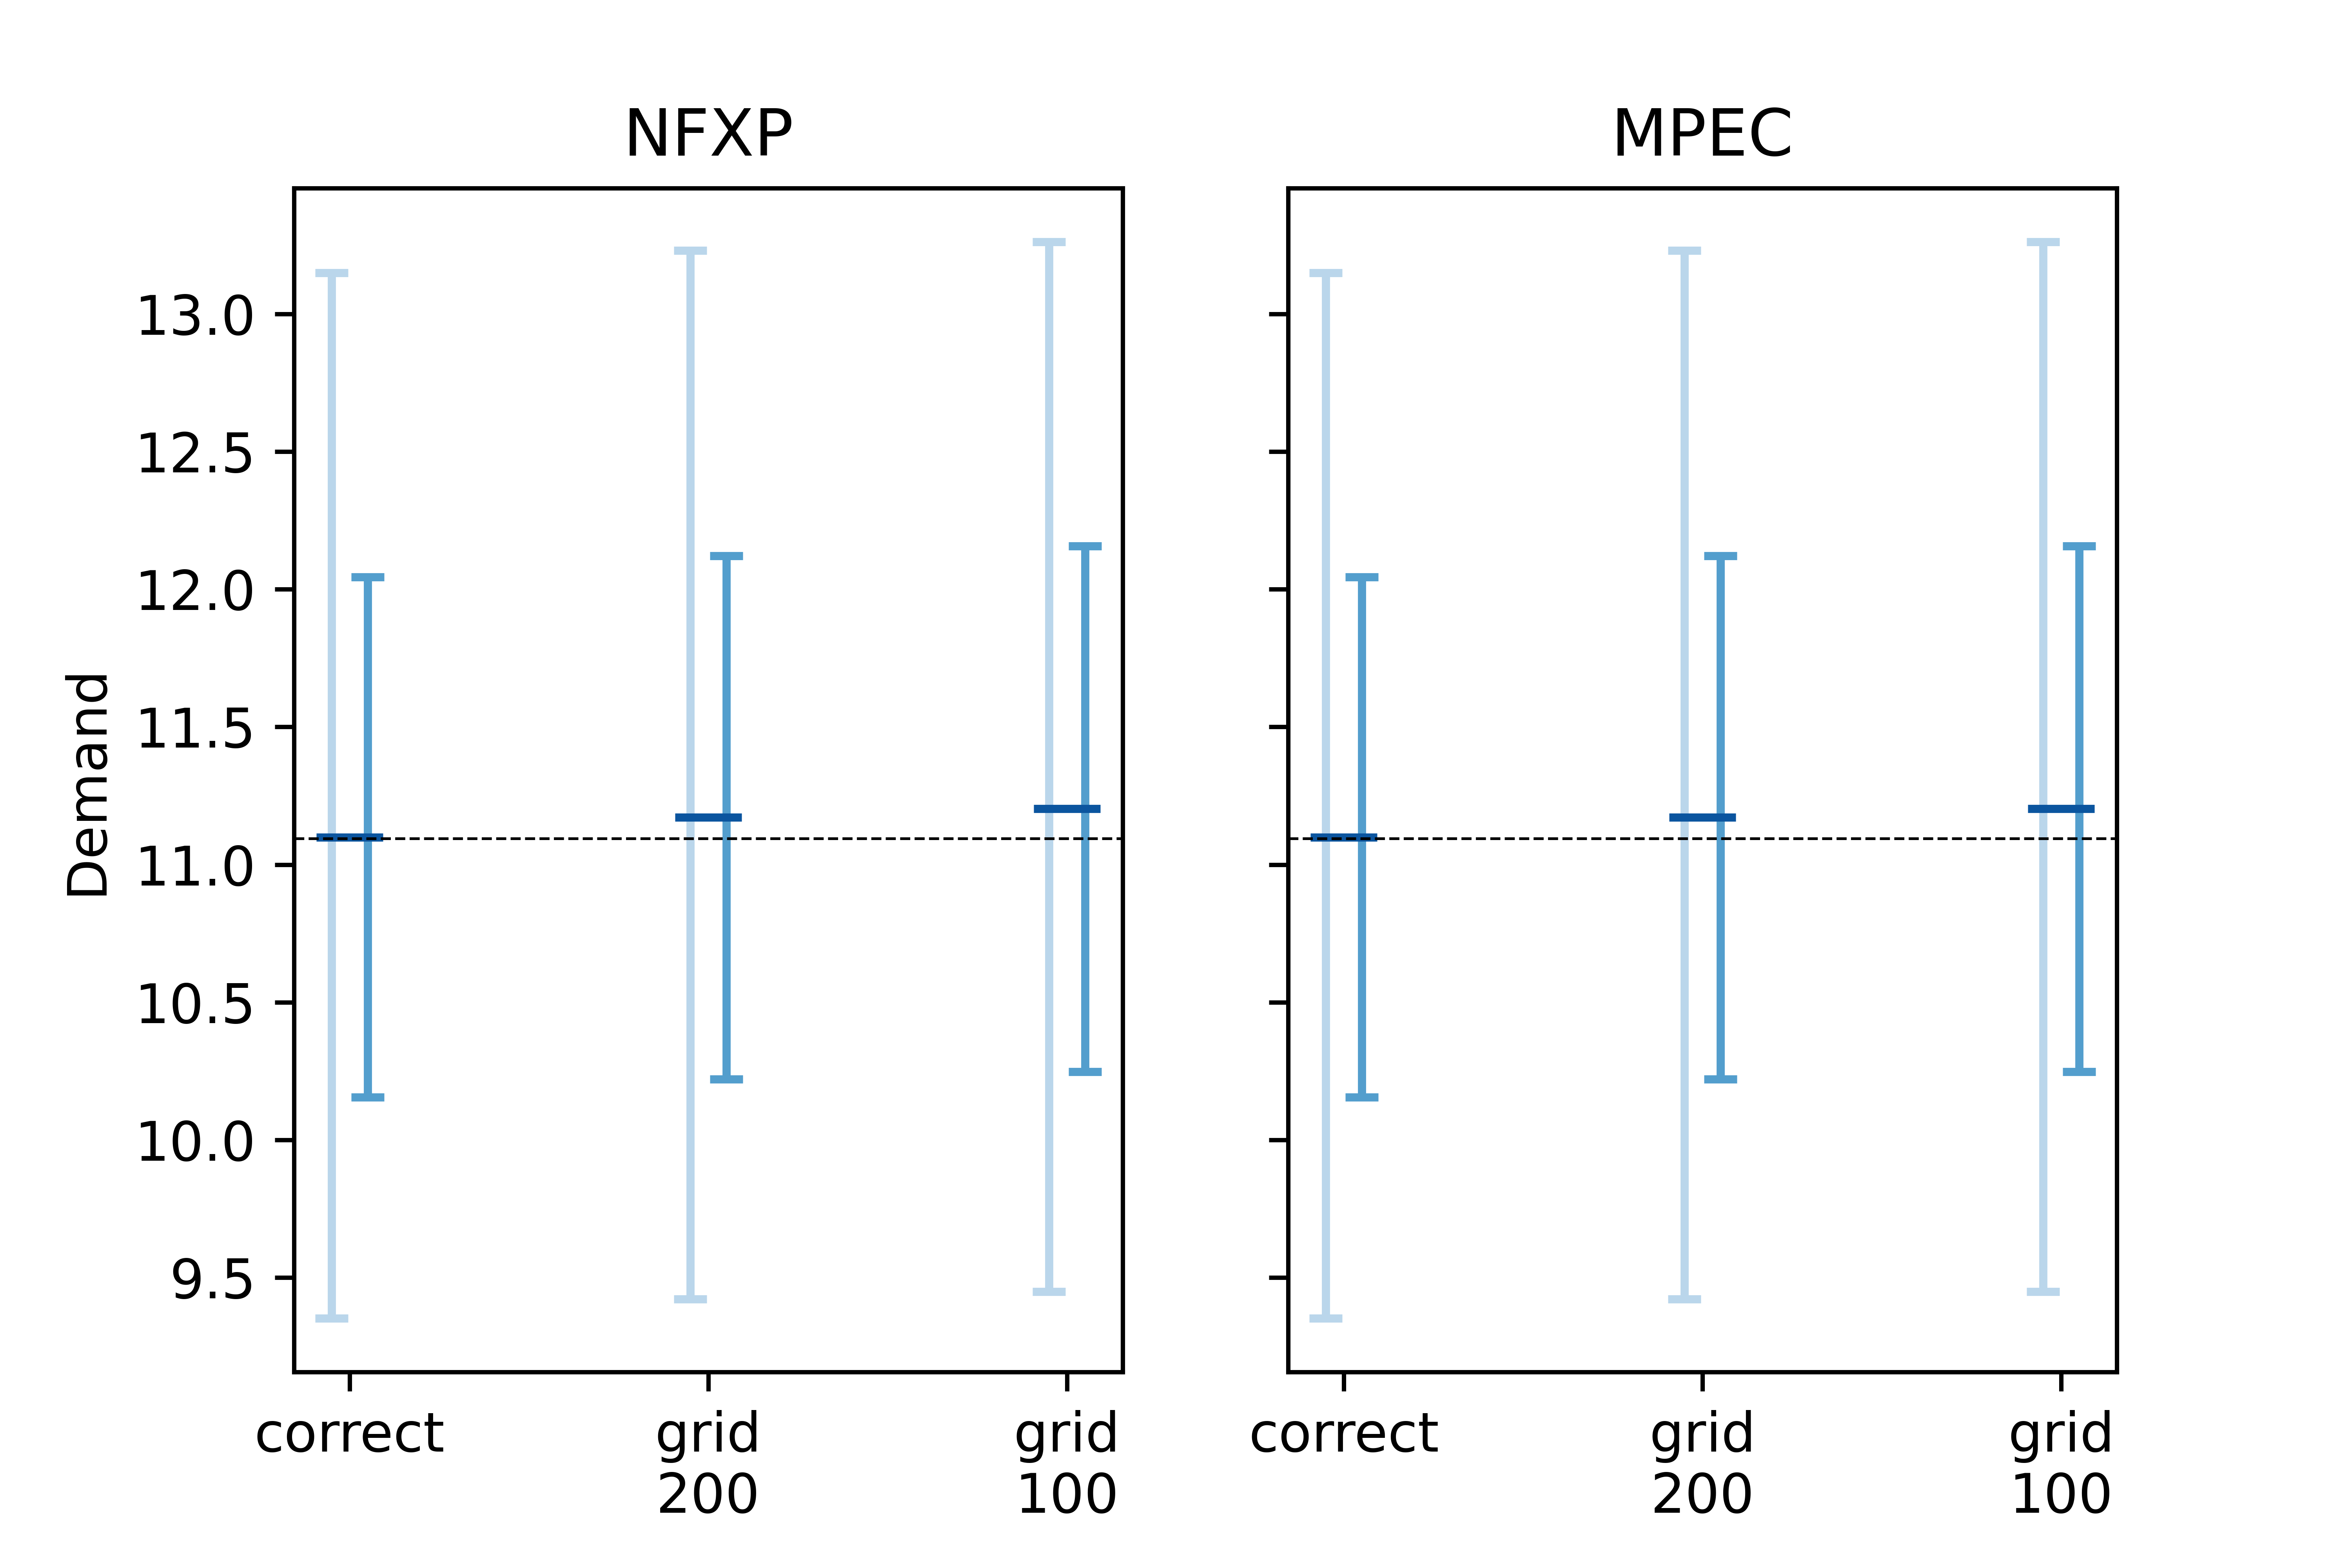
\includegraphics[scale=0.9]{../figures/figure_7.png}
	\label{figure7}
\end{figure}

\begin{figure}[H]
	\caption{Distribution of the QoI}
	\vspace*{-4mm}
	\centering
	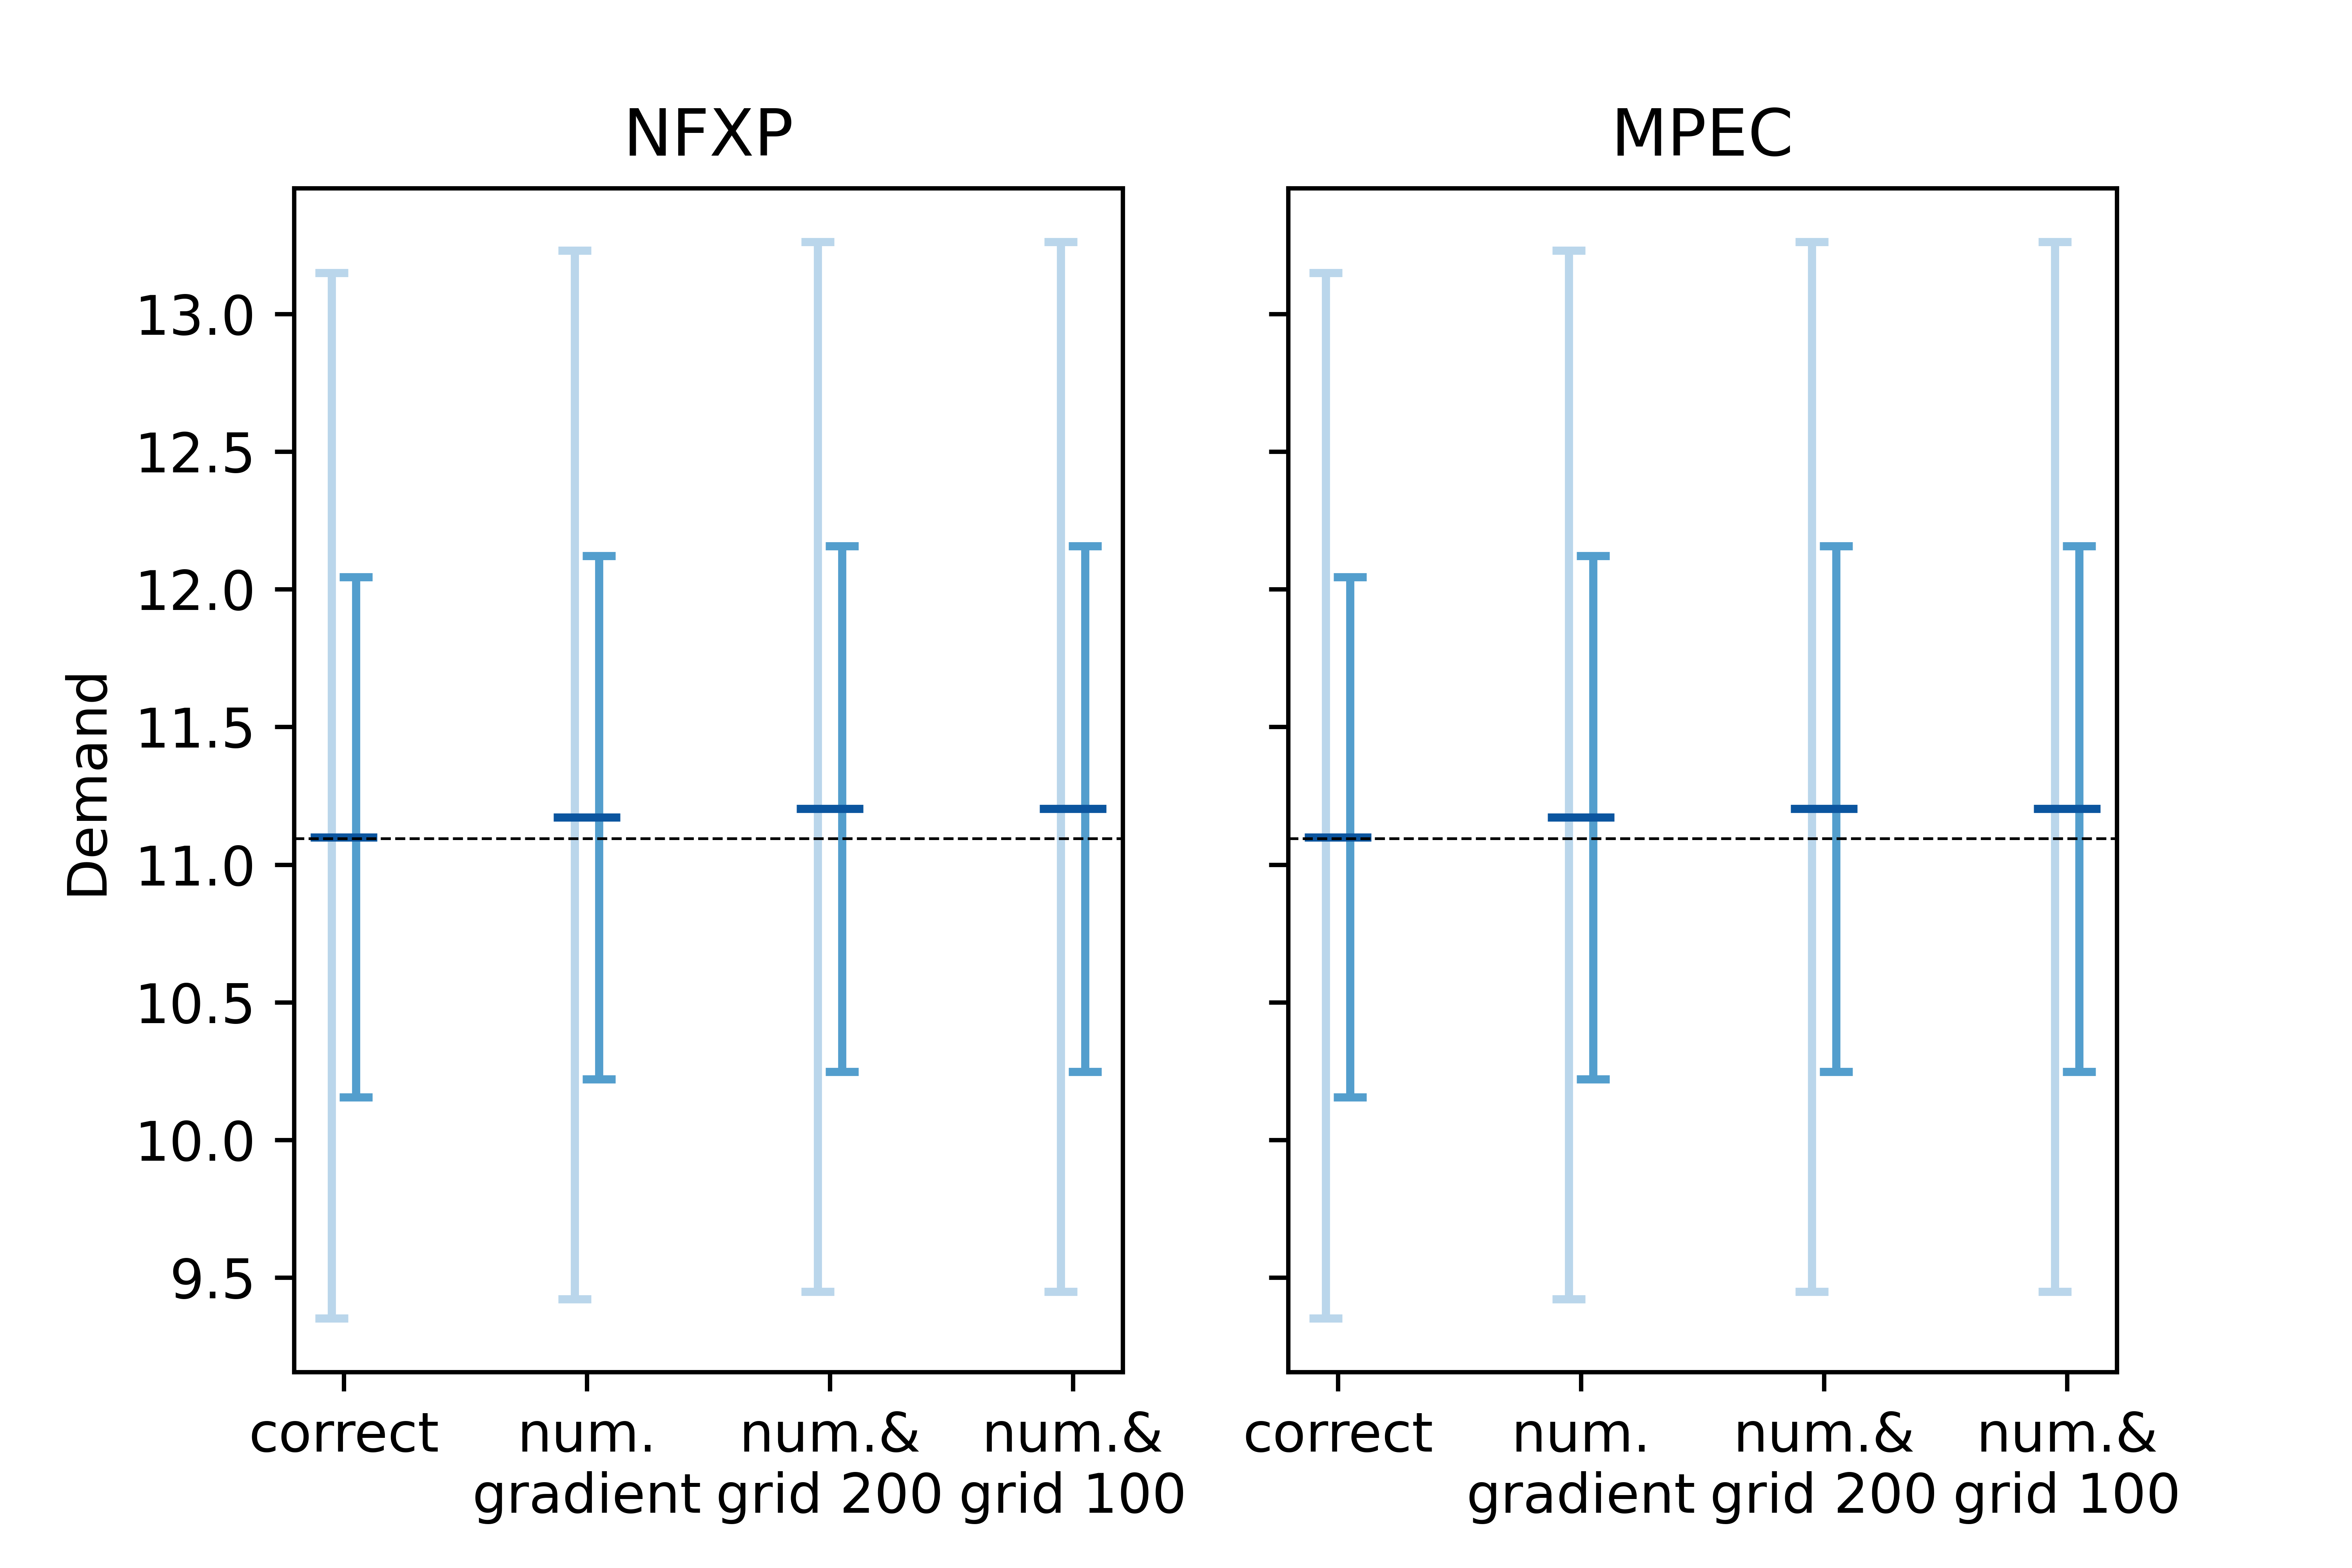
\includegraphics[scale=0.9]{../figures/figure_8.png}
	\label{figure8}
\end{figure}

\begin{figure}[H]
	\caption{Distribution of the QoI}
	\vspace*{-4mm}
	\centering
	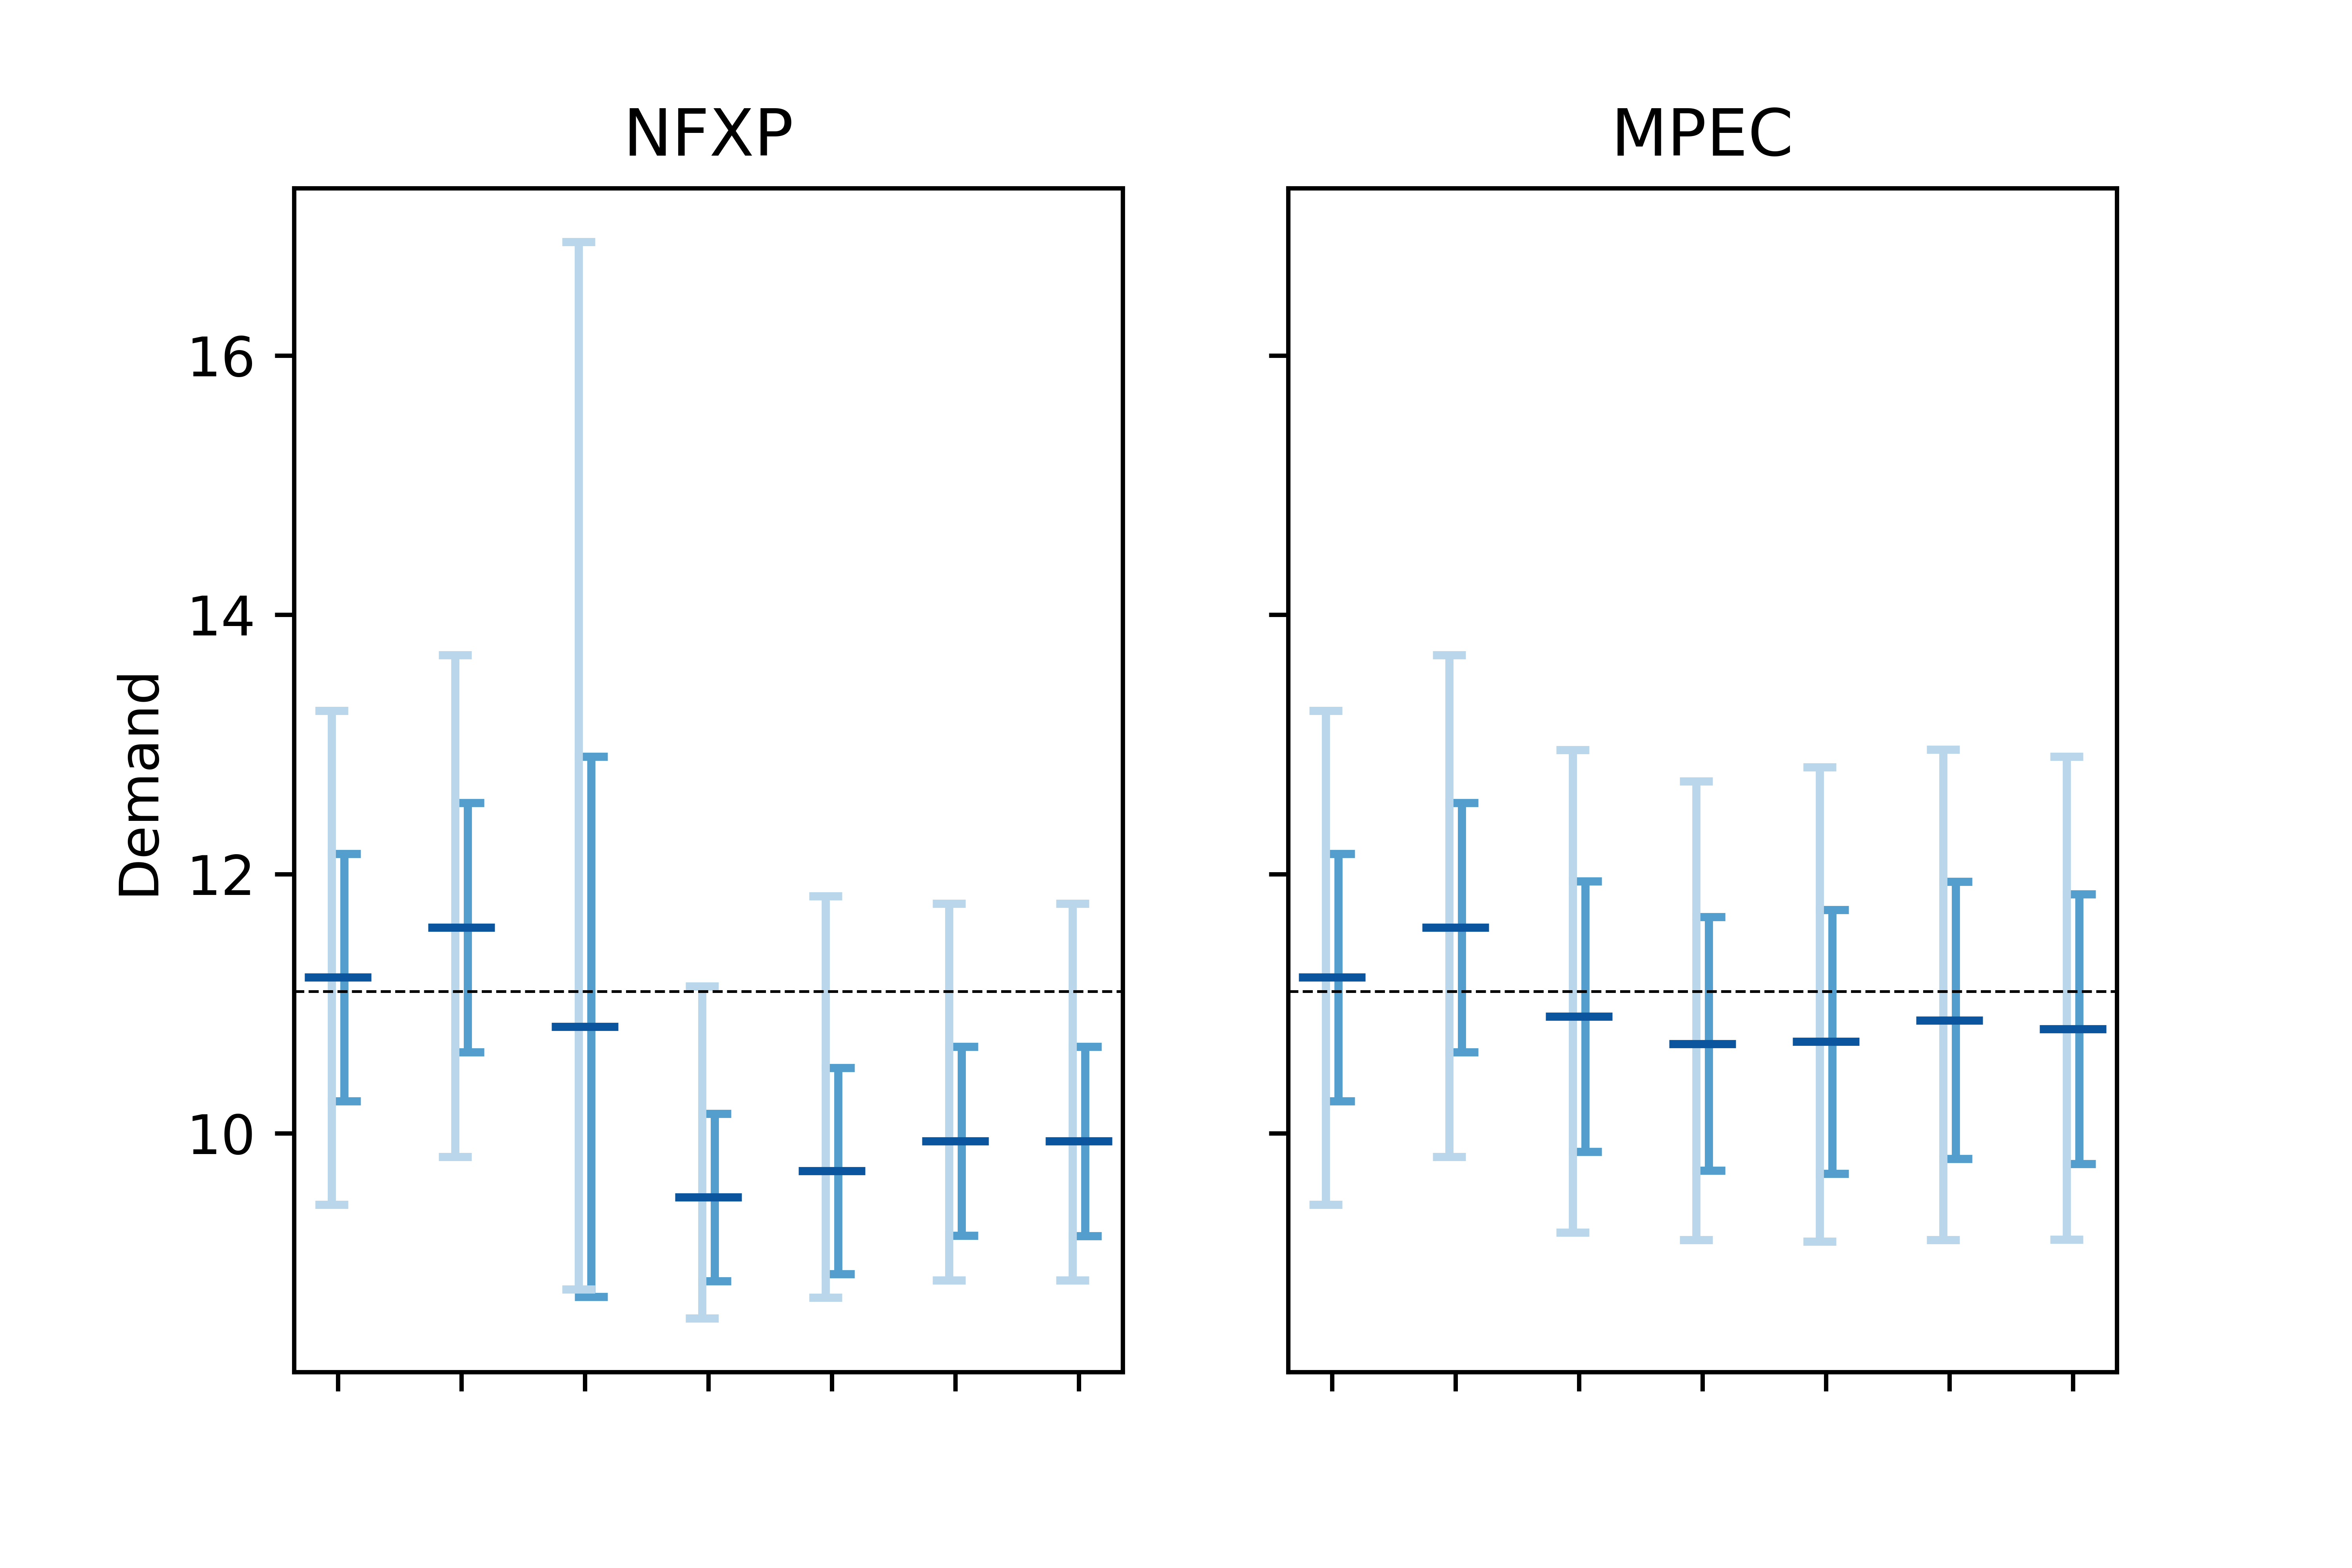
\includegraphics[scale=0.9]{../figures/figure_9.png}
	\label{figure9}
\end{figure}

\begin{figure}[H]
	\caption{Distribution of the QoI}
	\vspace*{-4mm}
	\centering
	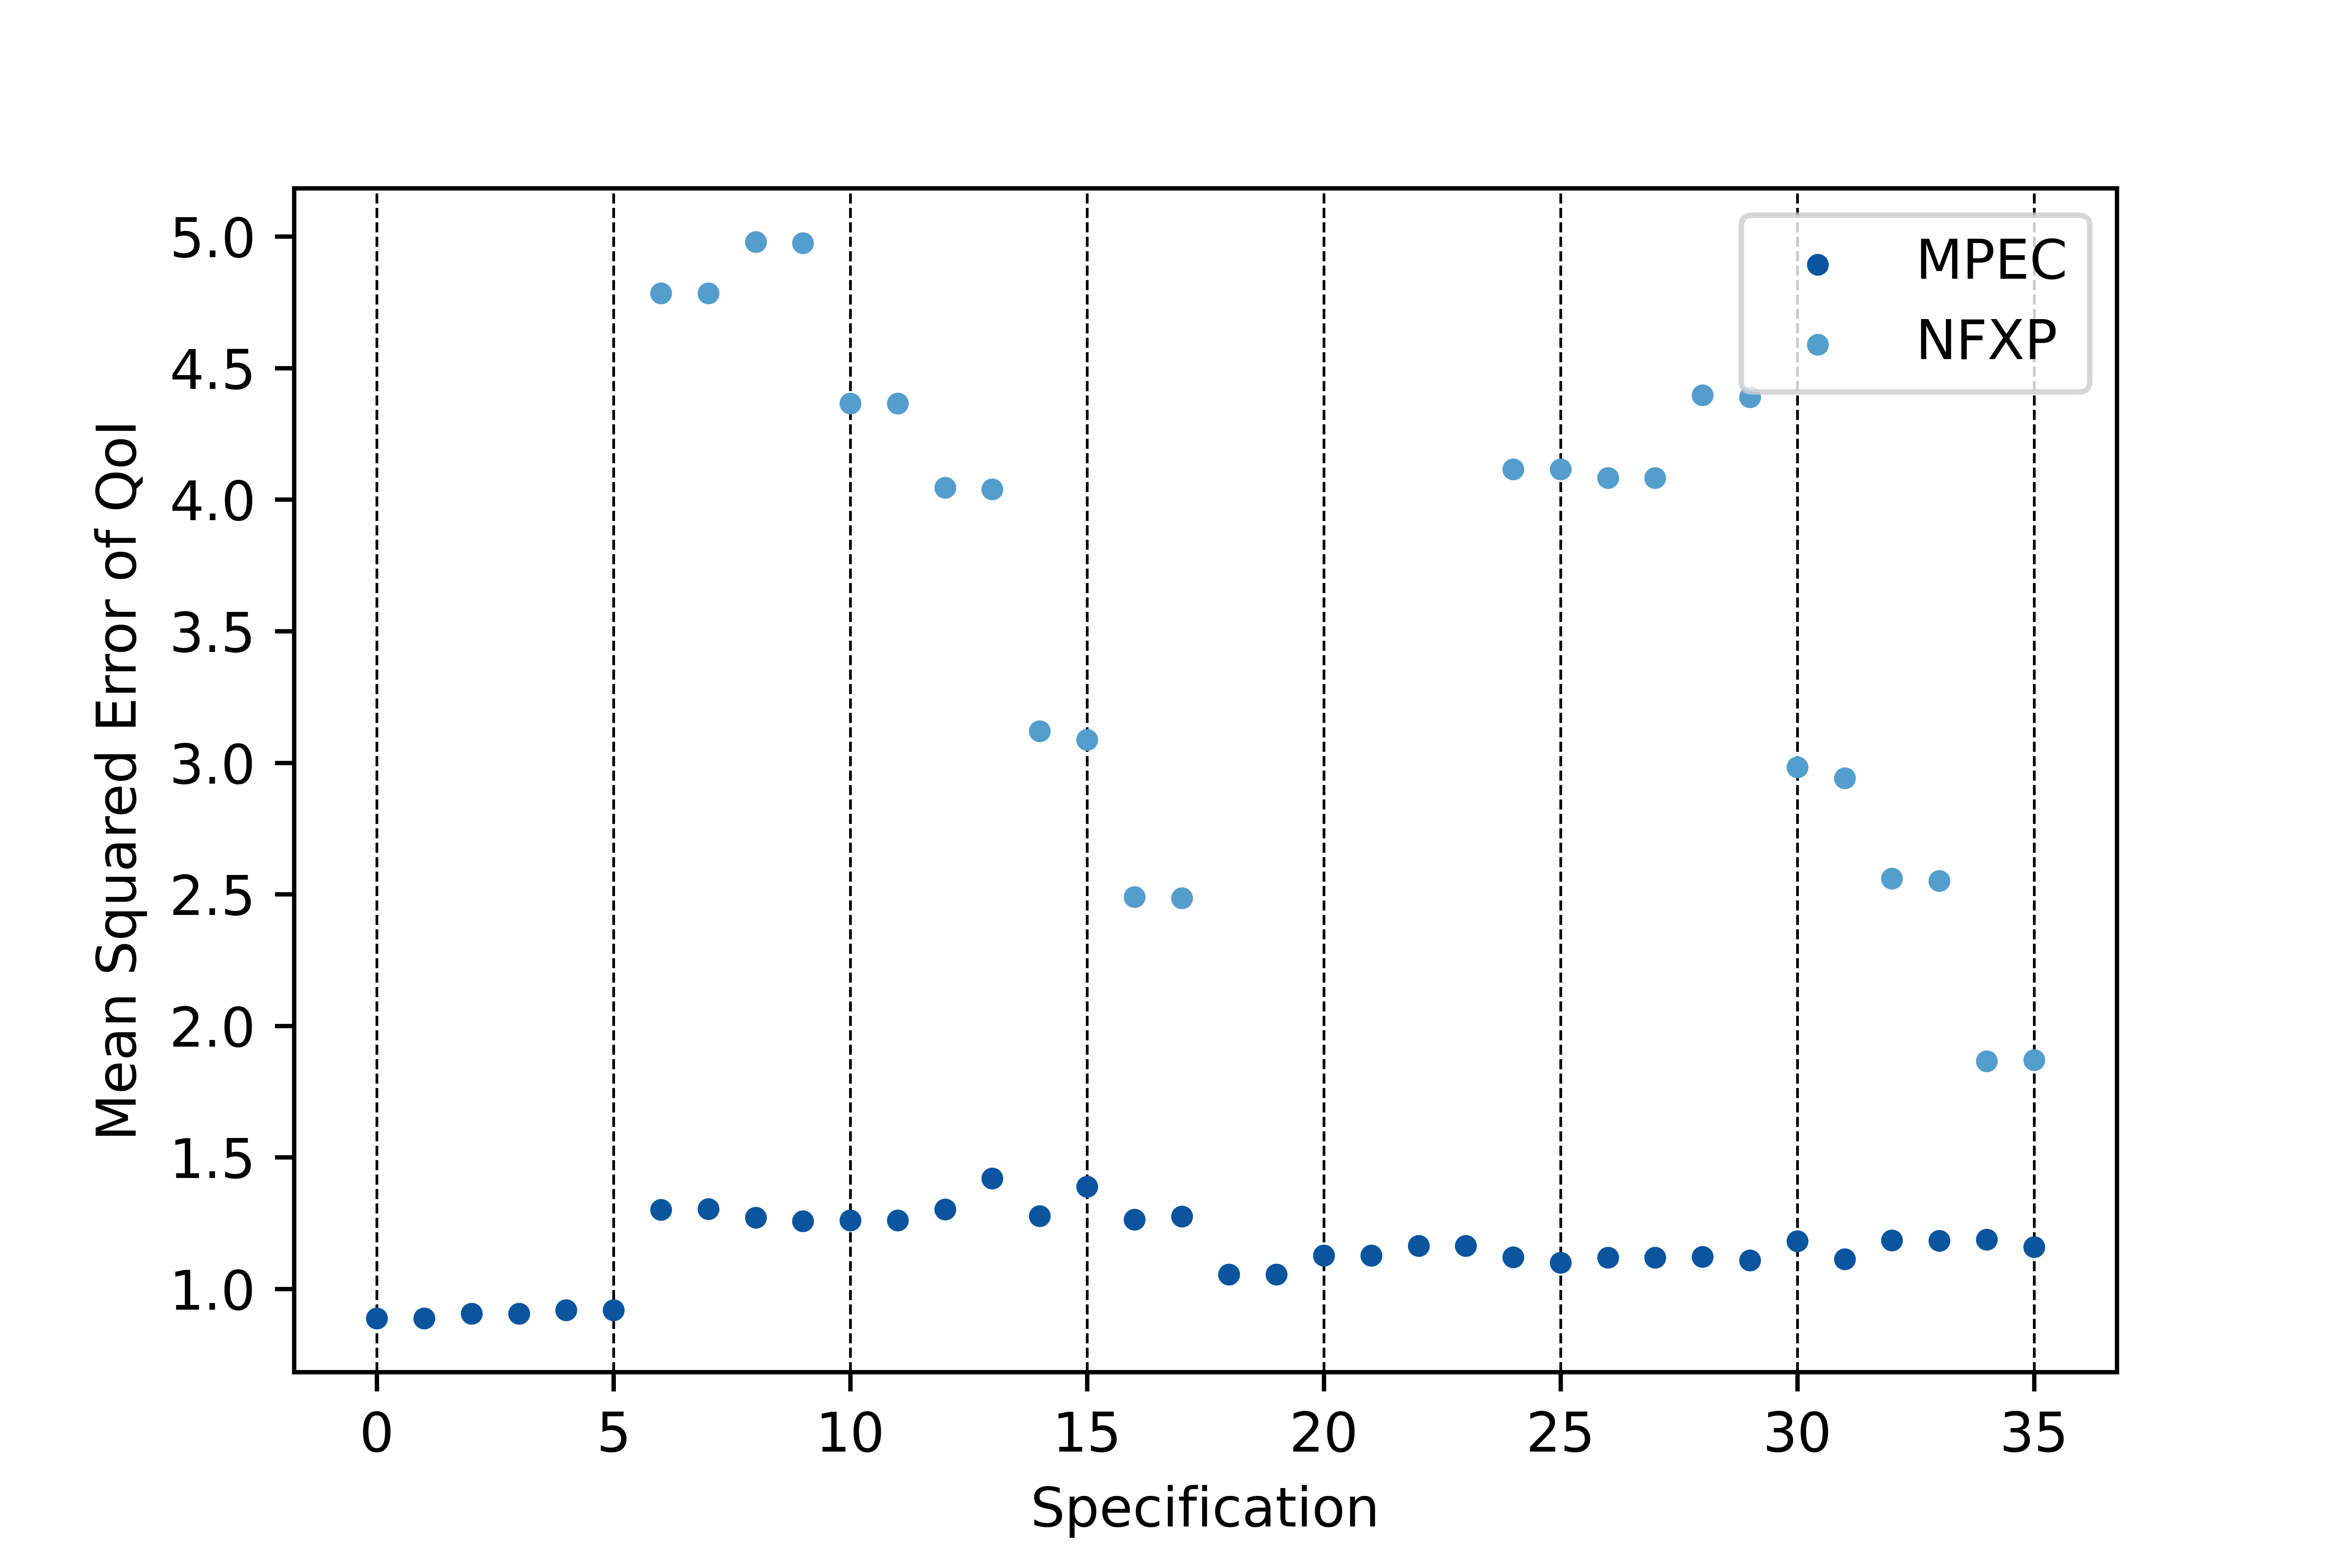
\includegraphics[scale=0.9]{../figures/figure_10.png}
	\label{figure10}
\end{figure}

\begin{figure}[H]
	\caption{Distribution of the QoI}
	\vspace*{-4mm}
	\centering
	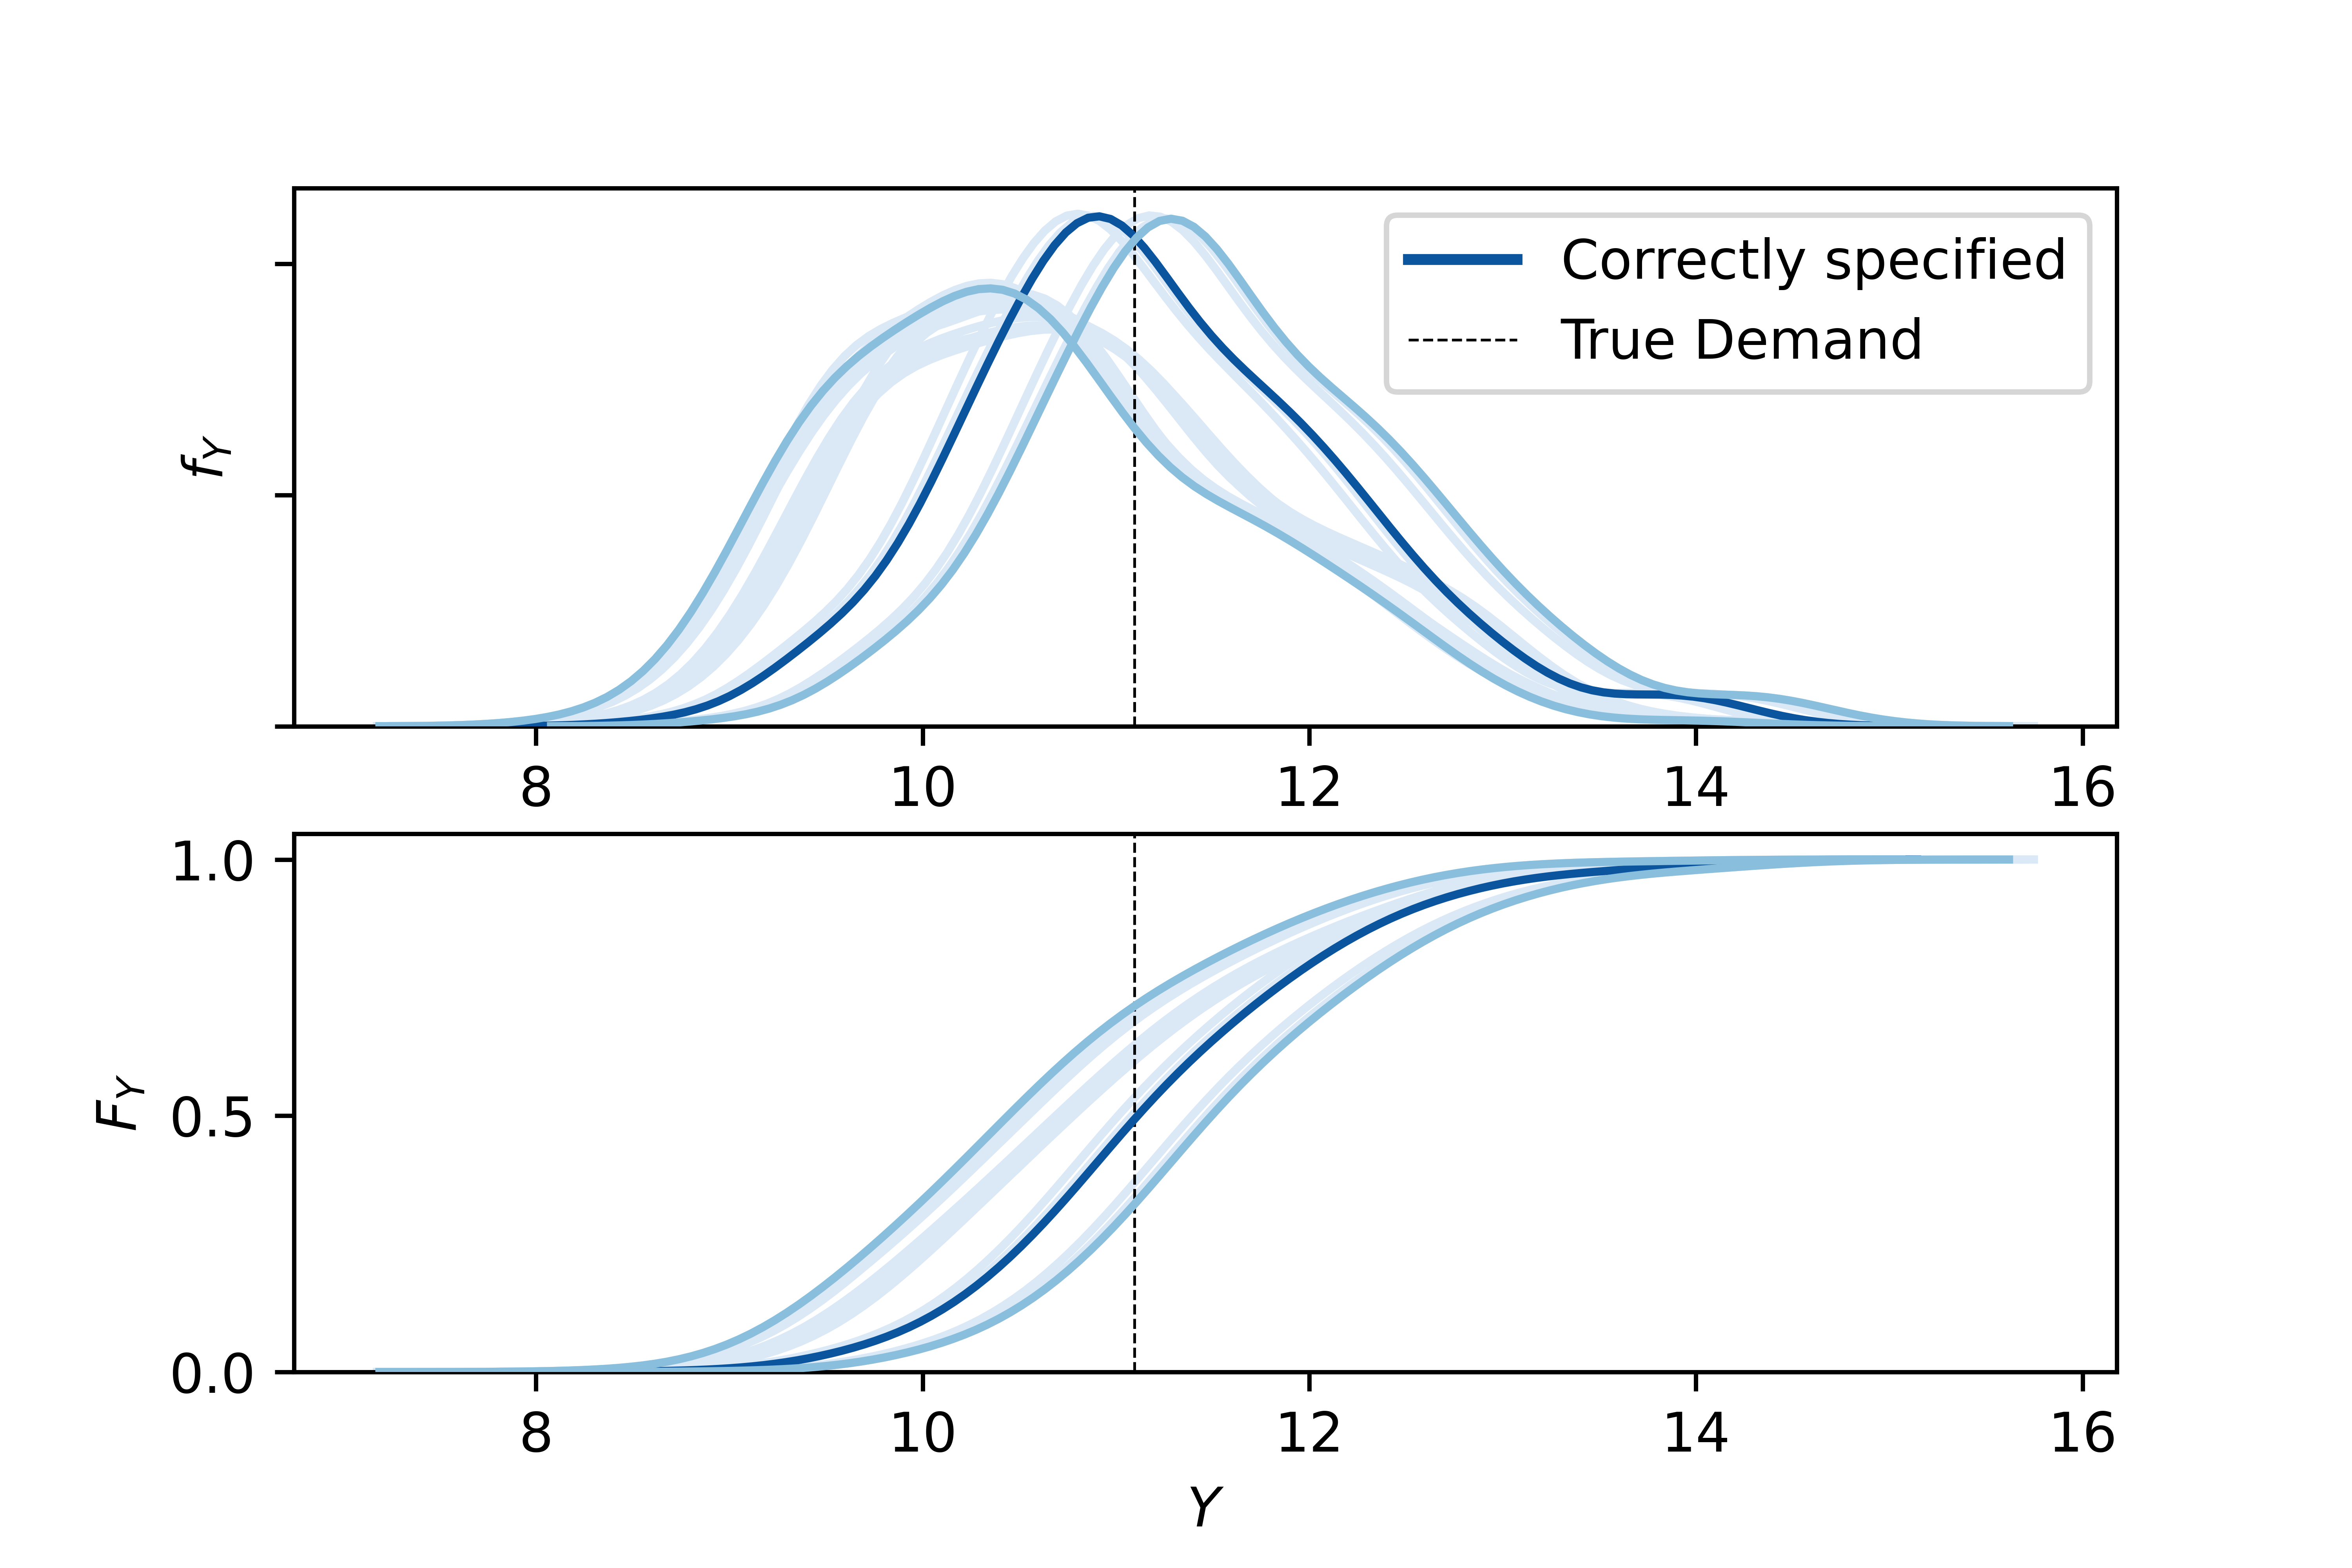
\includegraphics[scale=0.9]{../figures/figure_11.png}
	\label{figure11}
\end{figure}

\begin{figure}[H]
	\caption{Distribution of the QoI}
	\vspace*{-4mm}
	\centering
	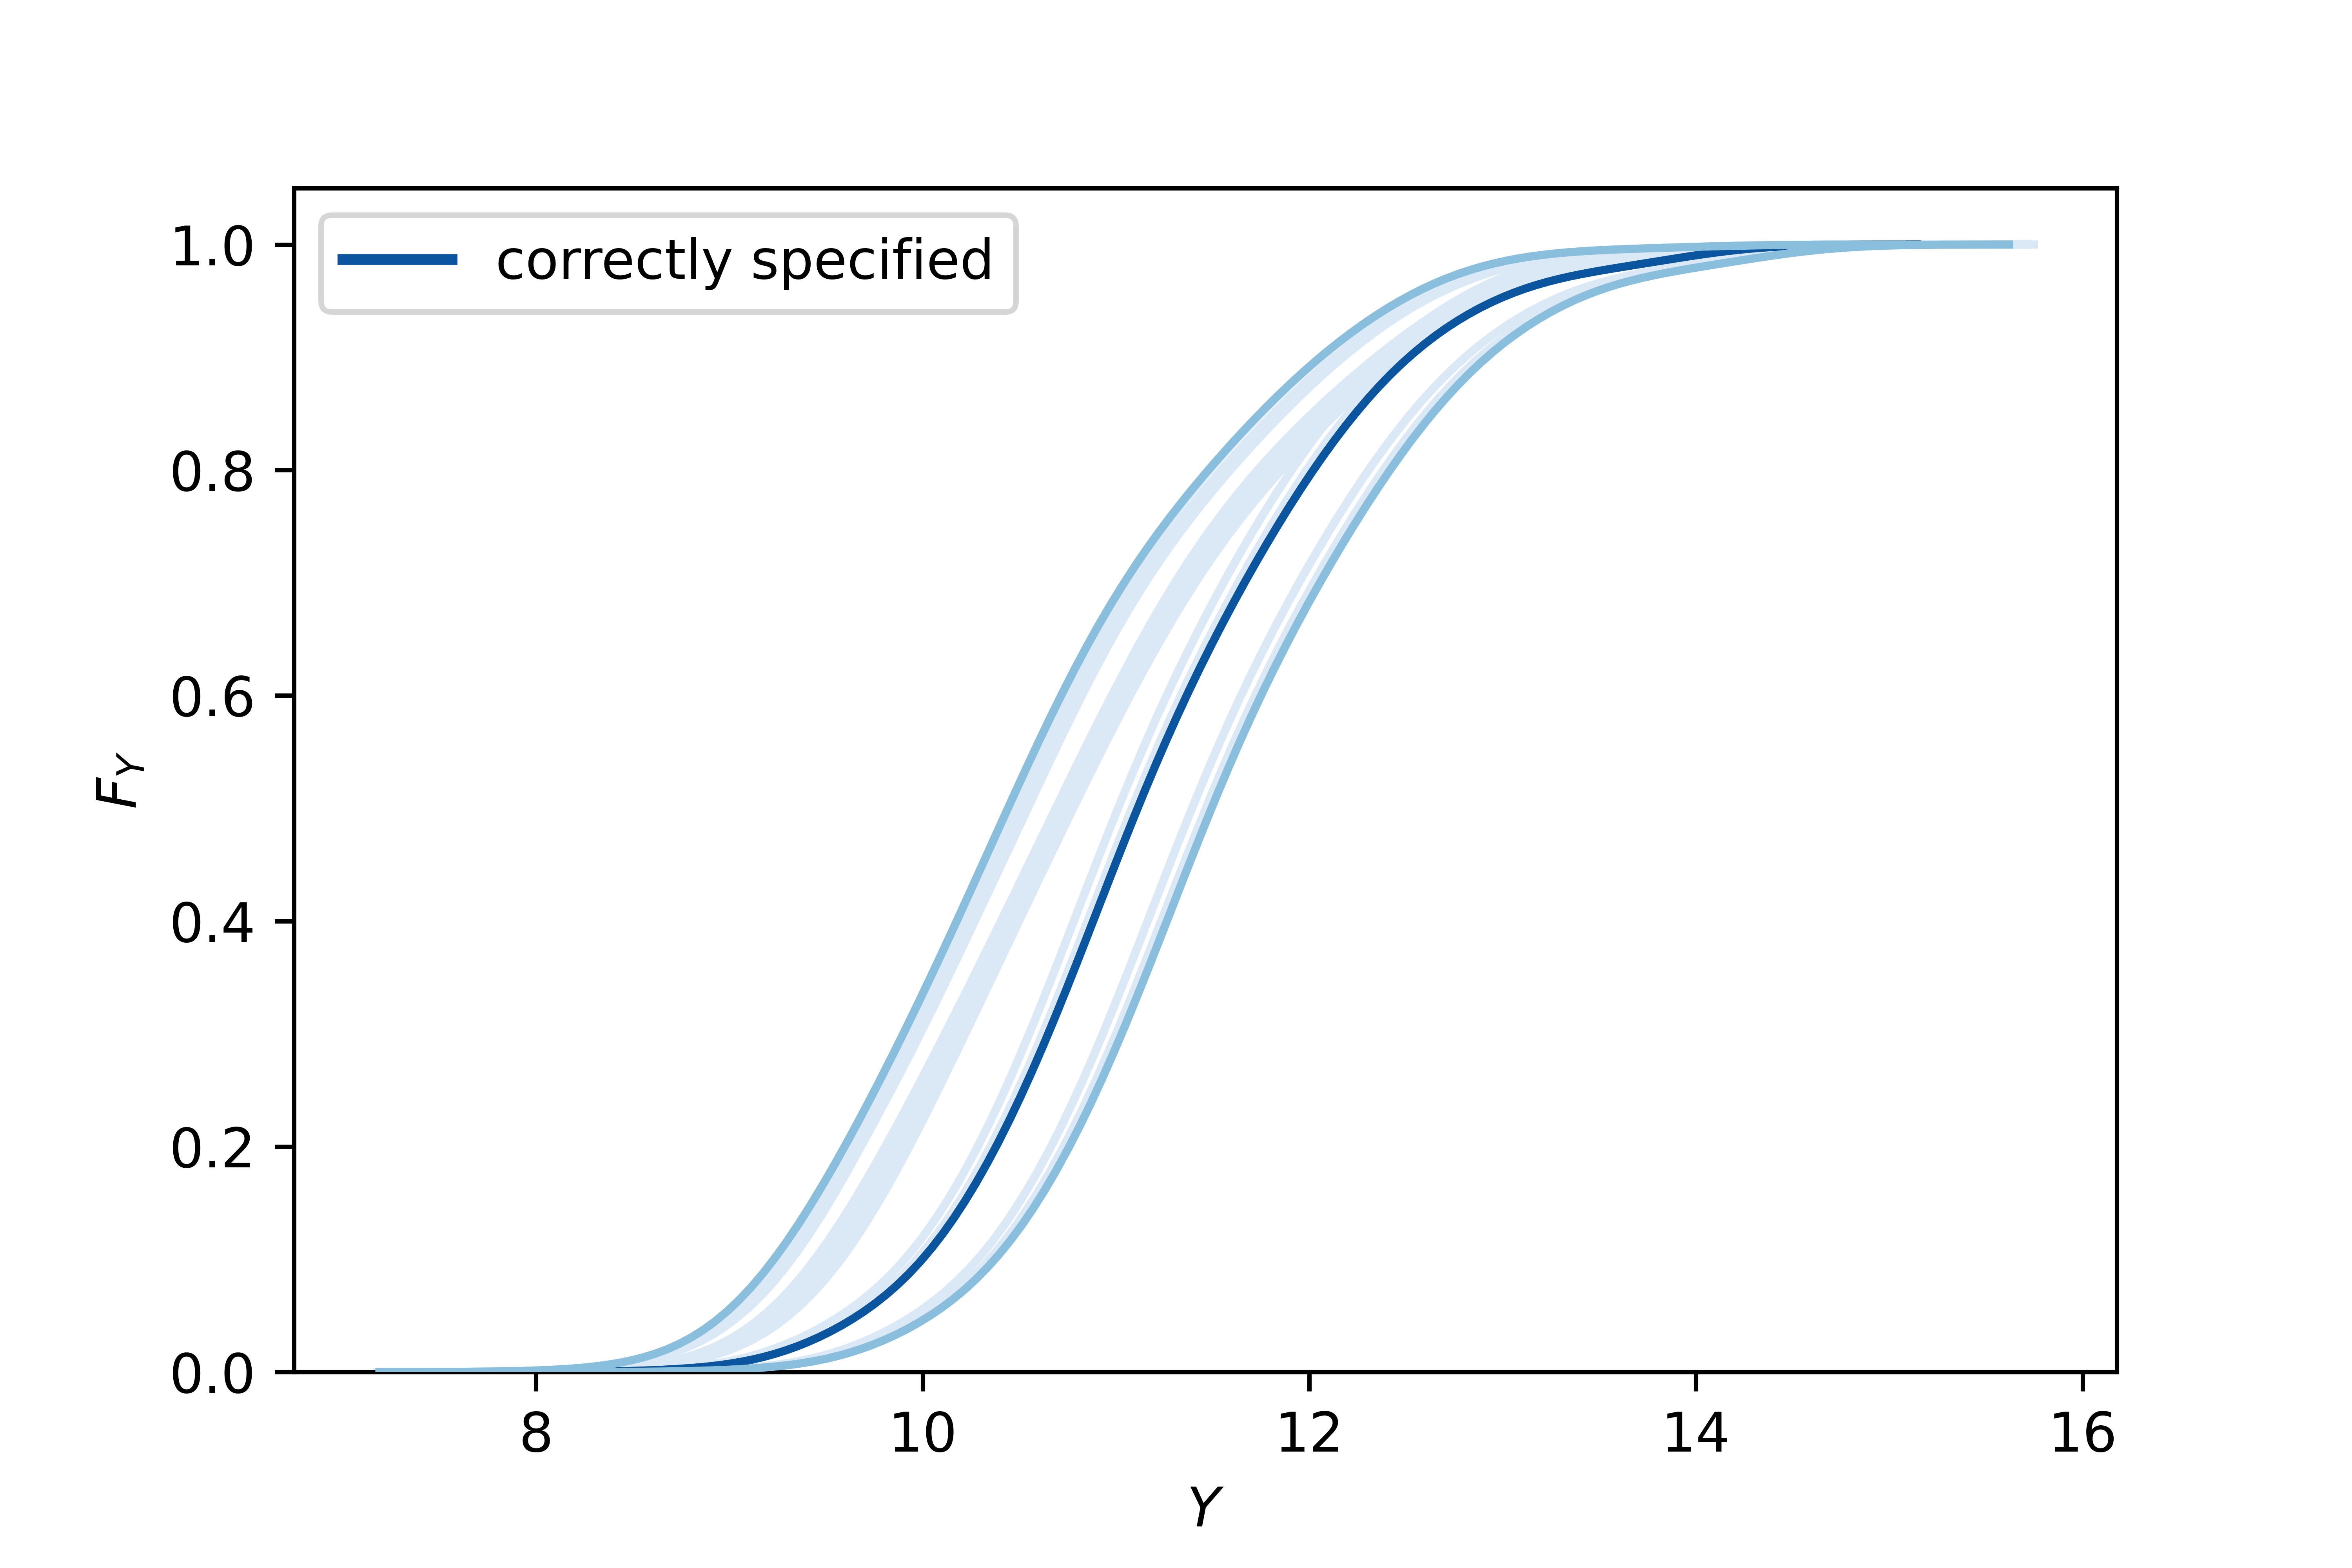
\includegraphics[scale=0.9]{../figures/figure_12.png}
	\label{figure12}
\end{figure}

\begin{figure}[H]
	\caption{Distribution of the QoI}
	\vspace*{-4mm}
	\centering
	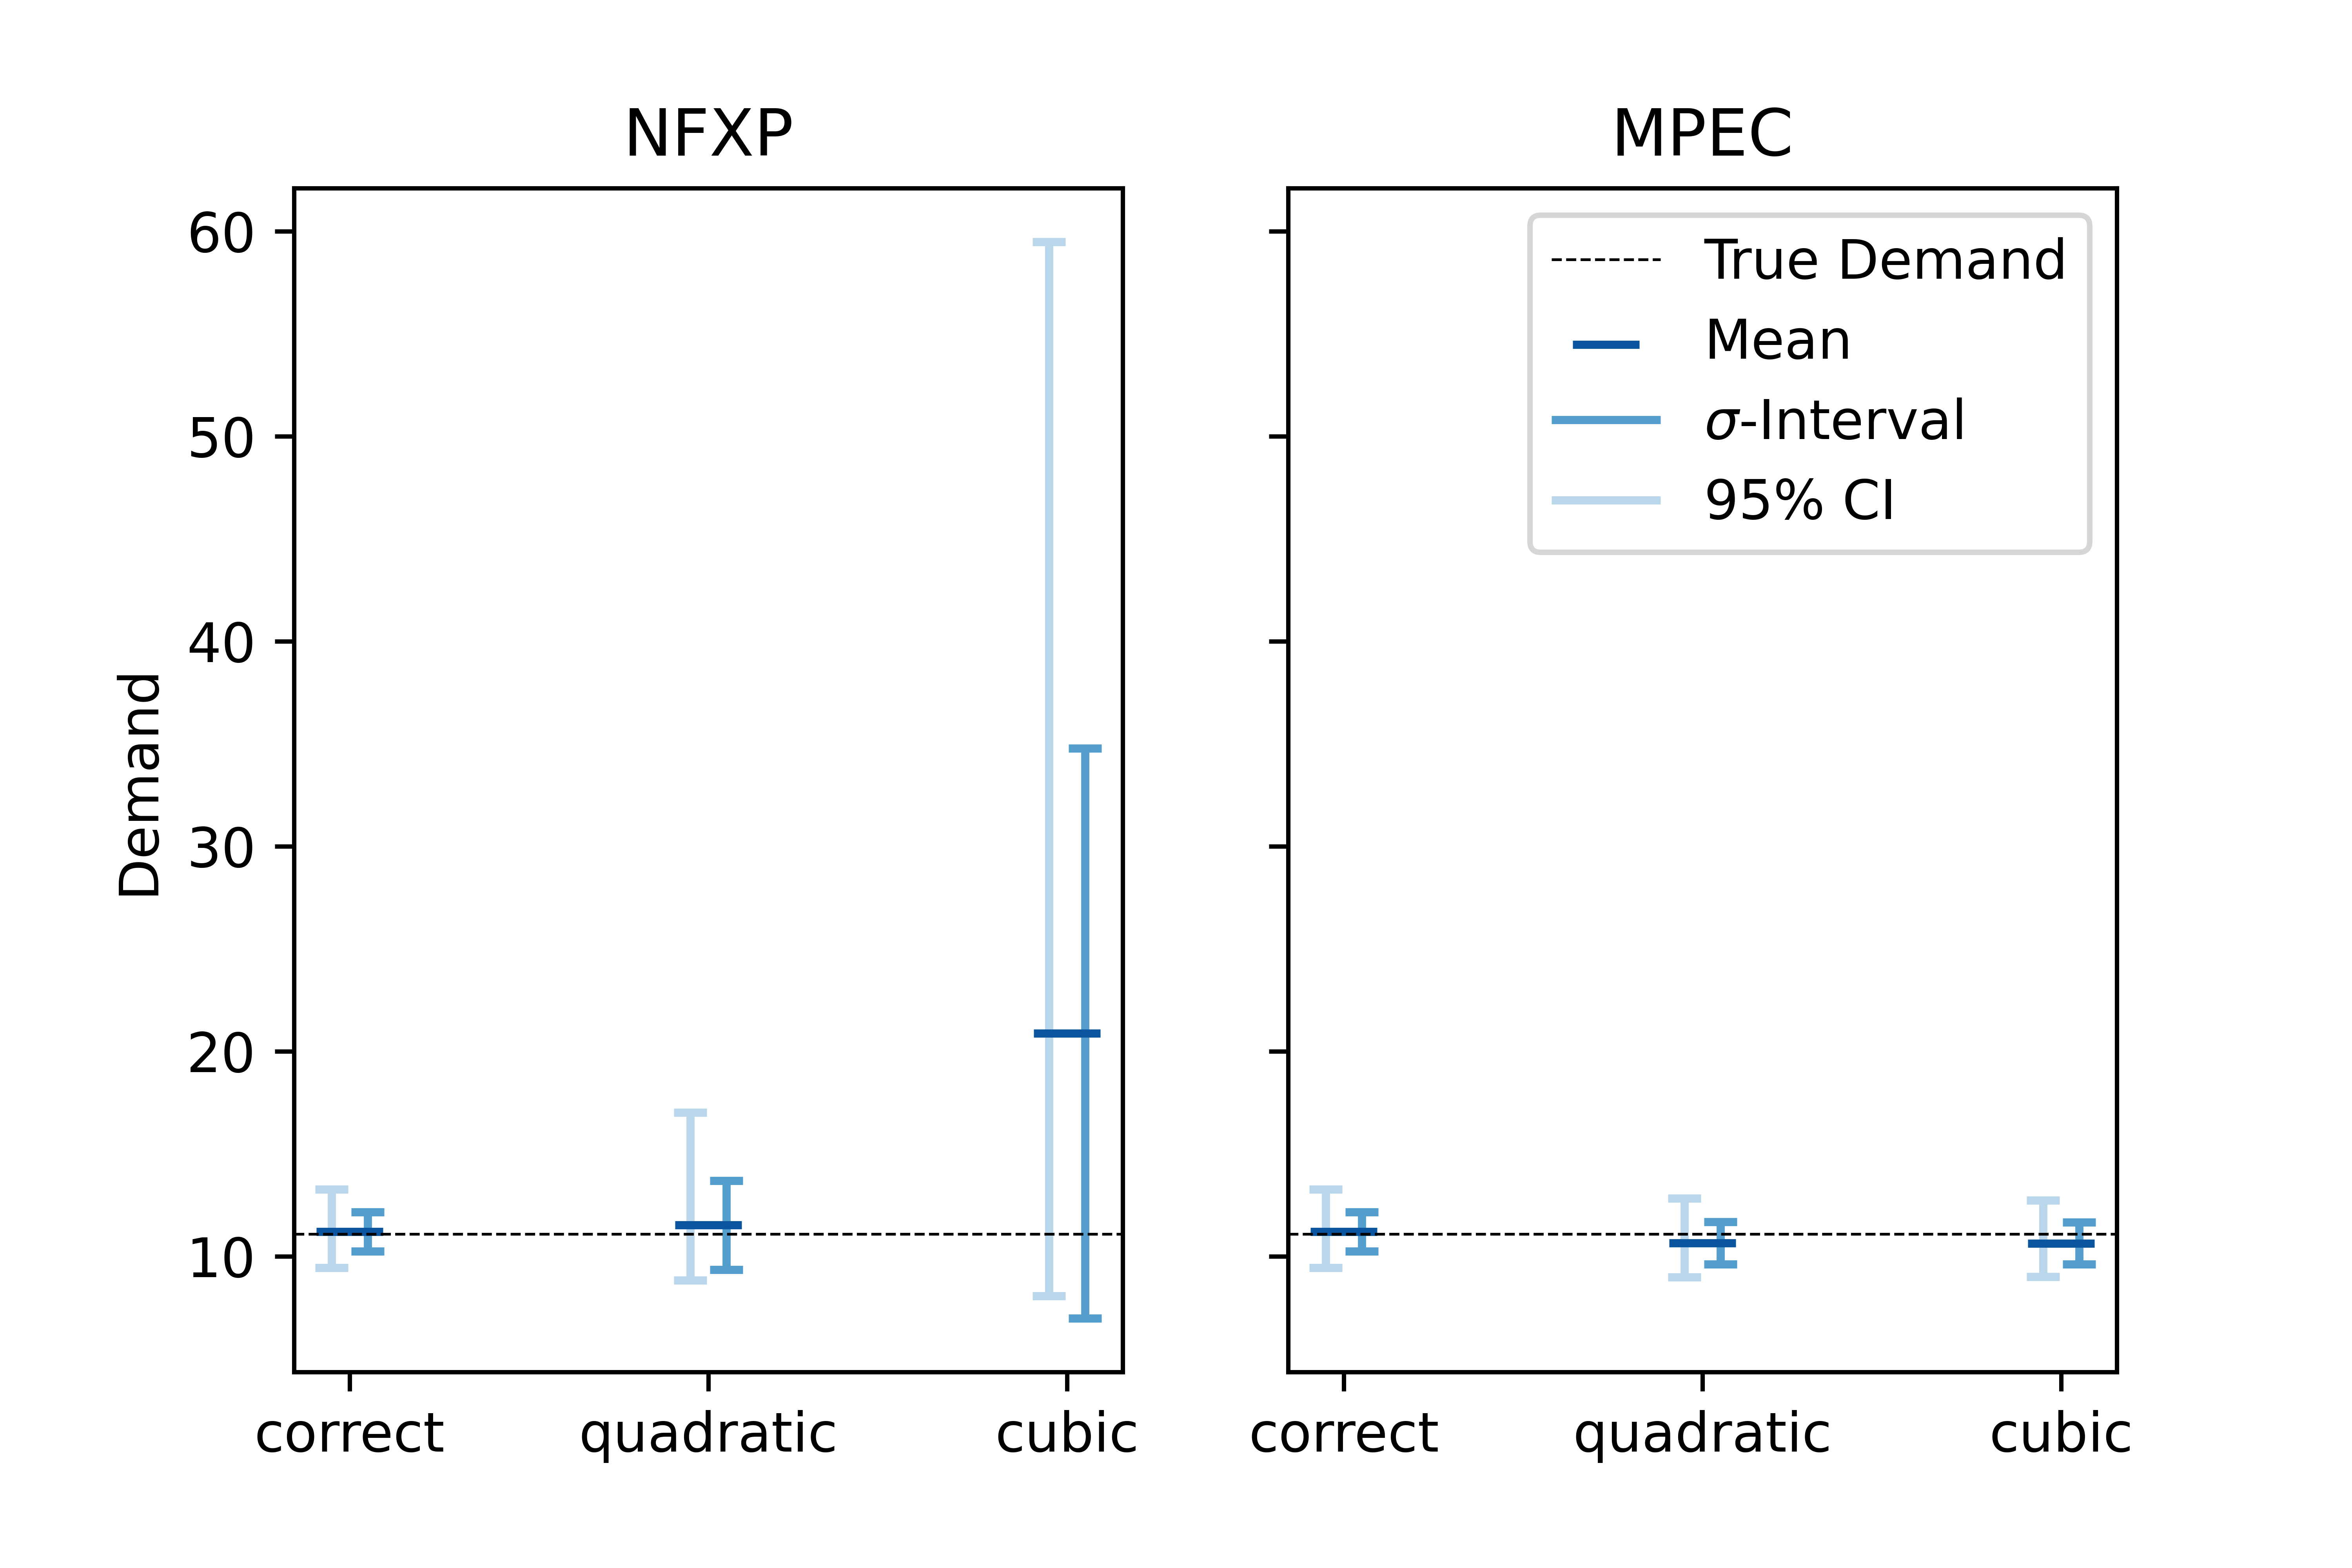
\includegraphics[scale=0.9]{../figures/figure_13.png}
	\label{figure13}
\end{figure}

